\documentclass[a4paper,12pt]{article}
\usepackage{cite}
\usepackage{braket}
\usepackage{amsmath}
\usepackage{graphicx}
\DeclareGraphicsExtensions{.png}
\usepackage{feynmf}
\usepackage{caption}
\usepackage{subcaption}
\usepackage{xcolor}
\usepackage{lineno}
\usepackage[margin=1in]{geometry}
\newcommand\todo[1]{\textcolor{red}{#1}}
\newcommand{\hgg}{$\textrm{H} \rightarrow \gamma\gamma$ }
\newcommand{\unit}[1]{\textrm{ #1}}
\begin{document}
\begin{fmffile}{fd}

\begin{center}
    \huge Higgs Decay to Two Photons and the High Granularity Calorimeter
\end{center}
\begin{center}
    \large Peter Hansen
\end{center}
\linenumbers

\section{Introduction}

The Compact Muon Solenoid (CMS) is a detector at the Large Hadron Collider (LHC) experiment.
One of the major goals of the experiment was a search for the Standard Model (SM) Higgs boson.
The Higgs decay to two photons channel had the potential of making high resolution measurement of the Higgs mass.
Here, we discuss the measurement and the outlook of this measurement using a new highly granular endcap calorimeter (HGCal) in future LHC upgrades to a higher luminosity and center of mass energy. 
\section{Theory}
\subsection{Higgs Mechanism}


The Higgs boson is a neutral scalar particle which was added to the standard model to provide a mechanism that explains the mass of the gauge bosons, $W^\pm$ and $Z$.
The Higgs mechanism does this while keeping the Lagrangian gauge invariant.
The model consists a complex scalar field doublet $\phi$ with a Lagrangian
\cite{peskin1995introduction}
\begin{equation}
    \mathcal{L} = (D_\mu)^\dagger (D^\mu)-V(\phi)
    \label{eq:lagrangian}
\end{equation}
where
\begin{equation}
    V(\phi) = -\lambda v^2 \phi^2 + \lambda\phi^4
    \label{eq:potential}
\end{equation}
where $m_H = \sqrt{2\lambda}v$ and
\begin{equation}
    D_\mu = \partial_\mu + i \frac{g}{2} \vec \sigma \cdot \vec W_\mu + i \frac{g'}{2} B_\mu
\end{equation}
where $\vec W_\mu$ and $B_\mu$ are, respectively, the $SU(2)$ and $U(1)$ gauge bosons with $g$ and $g'$ coupling constants.
The potential has infinite degenerate minima with a vacuum expectation of
$\braket{0|\phi|0} = \frac{1}{\sqrt{2}} \left(\begin{smallmatrix} 0 \\ v \end{smallmatrix}\right)$.
The masses of the gauge bosons can be found by evaluating the first term of \ref{eq:lagrangian} at this minimum. 
\begin{equation}
    (D_\mu \phi) (D^\mu)^\dagger = \frac{1}{2}\left(\frac{v}{2}\right)^2 \left[ g^2(W_\mu^{(1)})^2 + g^2(W_\mu^{(2)})^2 + (-gW_\mu^{(3)} + g'B_\mu)^2 \right]
\end{equation}
The four vector fields can then be labeled 
\begin{align}
    W_\mu^\pm = \frac{1}{\sqrt{2}}(W_\mu^{(1)} \mp i W_\mu^{(2)}) & & m_W = \frac{gv}{2} \\
    Z_\mu^0 = \frac{gW_\mu^{(3)} - g' B_\mu)}{\sqrt{g^2+g'^2}} & & m_Z = \sqrt{g^2 + g'^2}\frac{v}{2} \\
    A_\mu = \frac{gW_\mu^{(3)} + g' B_\mu)}{\sqrt{g^2+g'^2}} & & m_A = 0
\end{align}

This leaves four free parameters in the model, the coupling constants $g$ and $g'$, and the Higgs potential constants $v$, and $\lambda$.
From measurements of $M_W$ and $g$, we get $v= 246$ GeV.
A measurement of the Higgs mass defines $\lambda$ through $M_H^2 = 2\lambda v^2$. 
\subsection{Higgs Decay}

The Standard Model Higgs couples to fermions with a interaction vertex proportional to the fermion mass, $-im_f/v$, $W$ bosons with $gm_W$, and $Z$ bosons with $g' m_Z$.
It will decay to any fermion where $m_H > 2m_f$ and to the $W$ and $Z$ bosons if $m_H$ is sufficiently large, preferring the most massive kinematically possible decays.
However, decays to massless particles, \hgg and $H \rightarrow gg$ are possible through virtual loops of massive particles, shown in Figure \ref{fig:hdiphoton}. 

\begin{figure}
    \centering
    
    \begin{subfigure}{.45\textwidth}
        \begin{fmfgraph*}(160,120)
            \fmfleft{i}
            \fmfright{o1,o2}
            \fmf{dashes,label=$H$}{i,v1}
            \fmf{photon}{v2,o1}
            \fmf{photon}{v3,o2}
            \fmf{fermion,label=$f$,l.side=left}{v1,v2,v3,v1}
            \fmflabel{$\gamma$}{o1}
            \fmflabel{$\gamma$}{o2}
            \fmfforce{(.33w, .5h)}{v1}
            \fmfforce{(.67w, .75h)}{v2}
            \fmfforce{(.67w, .25h)}{v3}
            \fmfforce{(w, .75h)}{o1}
            \fmfforce{(w, .25h)}{o2}
        \end{fmfgraph*}
    \end{subfigure}
    \begin{subfigure}{.45\textwidth}
        \begin{fmfgraph*}(160,120)
            \fmfleft{i}
            \fmfright{o1,o2}
            \fmf{dashes,label=$H$}{i,v1}
            \fmf{photon}{v2,o1}
            \fmf{photon}{v3,o2}
            \fmf{boson,label=$W$,l.side=left}{v1,v2,v3,v1}
            \fmflabel{$\gamma$}{o1}
            \fmflabel{$\gamma$}{o2}
            \fmfforce{(.33w, .5h)}{v1}
            \fmfforce{(.67w, .75h)}{v2}
            \fmfforce{(.67w, .25h)}{v3}
            \fmfforce{(w, .75h)}{o1}
            \fmfforce{(w, .25h)}{o2}
        \end{fmfgraph*}
    \end{subfigure}
    \caption{\hgg Feynman Diagrams}
    \label{fig:hdiphoton}
\end{figure}

The invariant amplitude of the decay, \hgg,  is \cite{Marciano2012,Shifman1979} 
\begin{equation}
    \mathcal{M} = \frac{e^2g}{(4\pi)^2m_W}F\left( k_1 \cdot k_2 g^{\mu\nu} - k_2^\mu k_1^\nu \right)\epsilon_\mu(k_1) \epsilon_\nu(k_2)
    \label{eq:ampl}
\end{equation}
where $F$ is a sum over the $W$ and fermion loops
\begin{equation}
    F = F_W(\beta_W) + \sum_f N_c Q_f^2 F_f(B_f)
    \label{eq:F}
\end{equation}
where $B_W = 4m_W^2/m_H^2$, $B_f = 4m_f^2/m_H^2$ and 
\begin{align}
    F_W(\beta) &=  2 + 3 \beta + 3\beta(2-\beta)f(\beta) \label{eq:FW} \\
    F_f(\beta) &= -2\beta[1 + (1-\beta) f(\beta)] \\ 
\end{align}
with
\begin{equation}
    f(\beta) = \begin{cases}
        \arcsin^2(\beta^{-1/2}) & \beta \ge 1 \\
        -\frac{1}{4}\left[ \ln \frac{1+\sqrt{1-\beta}}{1-\sqrt{1-\beta}}-i\pi \right]^2 & \beta < 1 
    \end{cases}
\end{equation}
The boson and fermion loops contribute with opposite sign and the decay rate is
\begin{equation}
    \Gamma(\textrm{H} \rightarrow \gamma\gamma) = |F|^2 \left( \frac{\alpha}{4\pi} \right)^2 \frac{G_F m_H^3}{8\sqrt{2}\pi} \approx 10 \text{ keV}
\end{equation}
and branching ratio is $2.28\cdot10^{-3}$.
At $\sqrt{s} = $ 7(8) TeV the Higgs production cross section is 17.5(22.3) pb resulting in around one thousand \hgg events from the 2012 CMS data \cite{Dittmaier:2011ti}.
When $\sqrt{s} = $ 14 TeV, the production cross section for higgs increases by a factor of 2.5. With an increase in luminosity, 40,000 \hgg events would be expected in the first few years of running.
See Table \ref{tab:higgevents} for details. 

\begin{table}
    \centering
    \begin{tabular}{|c|c|c|c|c|}
        \hline
        $\sqrt{s}$ (TeV) & $\int \mathcal{L}$ (fb${}^{-1}$) & $\sigma_H$ (pb) & $N_H$ & $N_{H\rightarrow\gamma\gamma}$ \\
        \hline
        \hline
        7 & 5.1 & 17.5 & 8.9$\cdot 10^{4}$ & 200 \\
        \hline
        8 & 19 & 22.3 & 4.2$\cdot 10^{5}$ & 1,000 \\
        \hline
        14 & 300 & 58 & 1.7$\cdot 10^{7}$ & 40,000 \\
        \hline
    \end{tabular}
    \caption{Higgs crossection $\sigma_H$, number of Higgs events $N_H$, \hgg events $N_{H\rightarrow\gamma\gamma}$ by center of mass energy and integrated luminosity}
    \label{tab:higgevents}
\end{table}

\section{CMS Detector}
The CMS is a general purpose detector around the LHC at CERN, designed to make precision measurements of the Standard Model and search for new physics beyond the Standard Model.
The primary subdetectors arranged around the beam are, starting with the closest, the silicon tracker, the Electromagnetic Calorimeter (ECAL), the Hadronic Calorimeter (HCAL), the superconducting solenoid and the muon chambers. 
The coordinate system in this paper has the $z$-axis along the beam line, $\phi$ is the azimuthal angle and the pseudorapidity $\eta \equiv - \ln \left[ \tan\left( \theta/2 \right) \right]$ is a measure of the zenith angle $\theta$. 
\begin{figure}[h]
    \begin{center}
        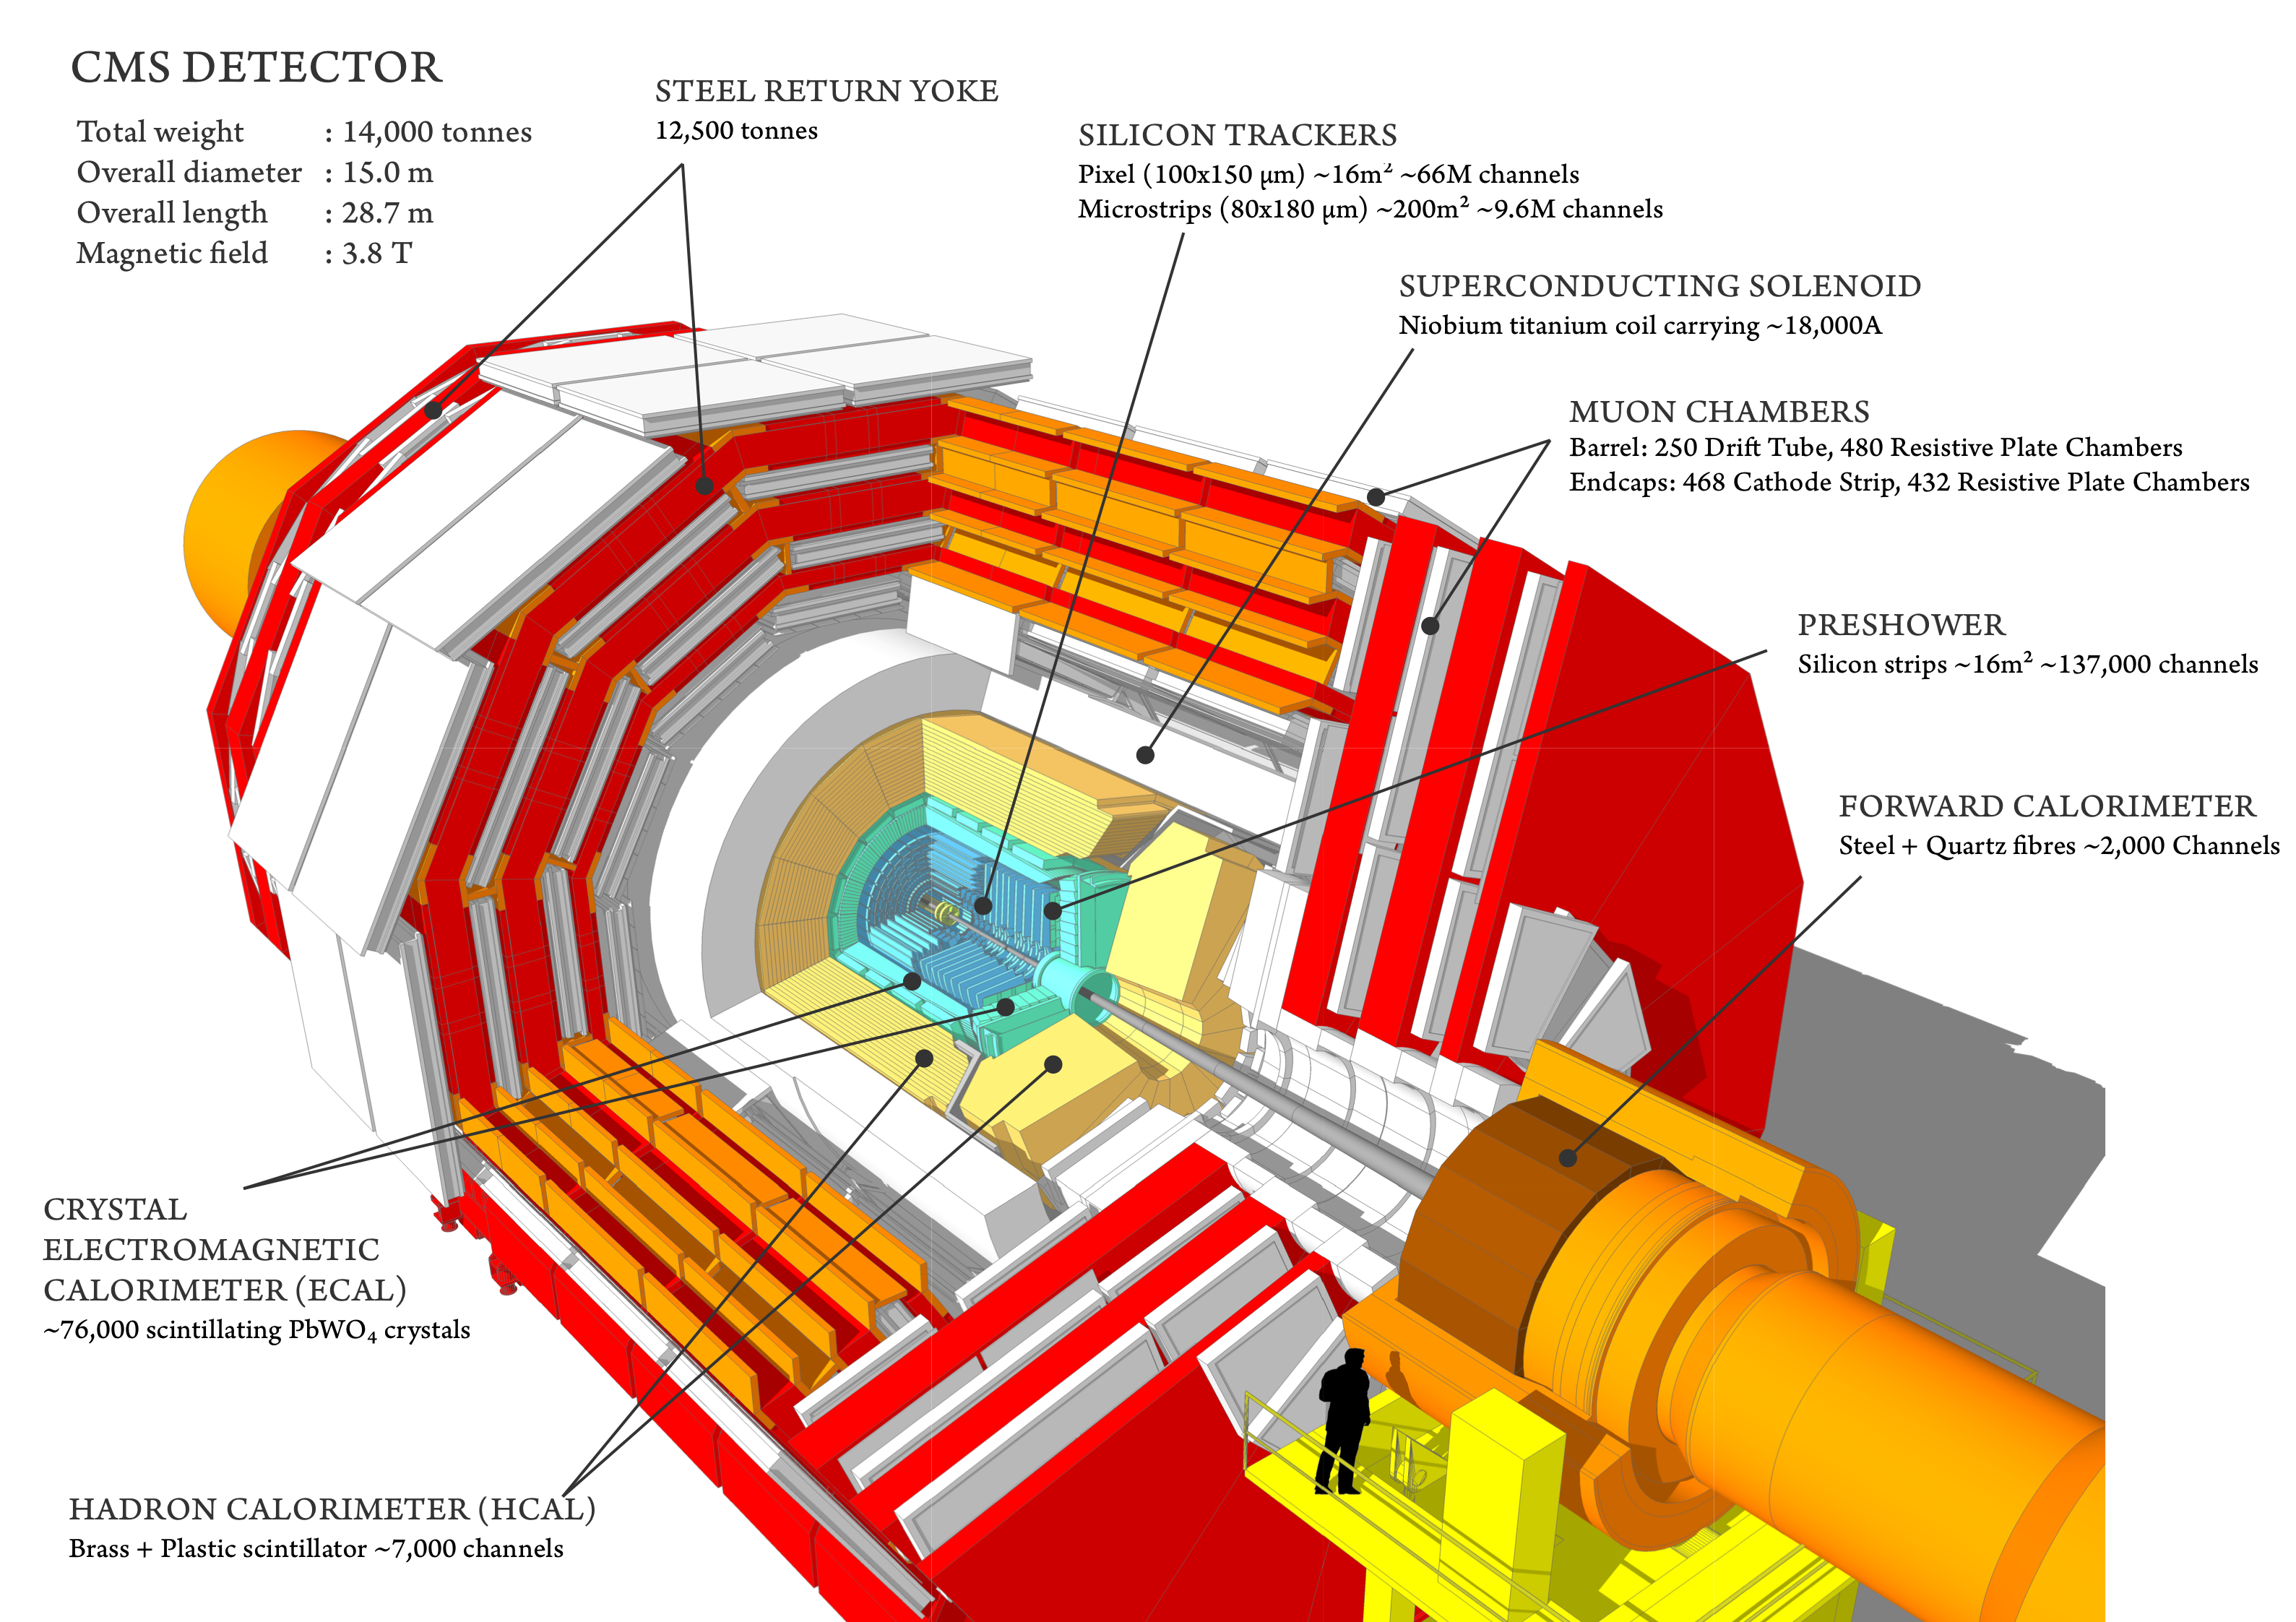
\includegraphics[width=\textwidth]{cms}
    \end{center}
    \caption{A cutaway view of the CMS Detector \cite{CMSFigure}}
    \label{fig:cms}
\end{figure}

The closest subdetector to the $pp$ interaction point is the silicon pixel and strip tracker which covers $|\eta| < 3$.
There are 66 million channels of 100x150$\mu$m pixels and 9.6 million channels for the 90x190$\mu$m strips.
As charged particles move through the layers of silicon, they deposit very small amounts of energy, allowing the tracker to reconstruct the path and origin of the particle.
The superconducting solenoid creates a 3.8 T magnetic field, curving the path of the charged particles and distinguishing the charge. 

The momentum of electrons and photons from the event are detected in the electromagnetic calorimeter (ECAL).
It is made of 76,000 lead tungstate scintillating crystals.
Particles travel through the transparent crystal energizing atoms which fluoresce at optical frequencies.
This scintillation light is detected and converted to a measurement of the energy deposited in the crystal.
Matched tracks in the tracker separate electrons from photons completing the picture of electromagnetic showers in ECAL.

Behind ECAL is the brass and plastic scintillator sampling hadronic calorimeter (HCAL).
The layers of brass absorber start the hadronic showers and each layer reduces the number of particles in the shower while plastic scintillator provides the energy signal.
The total energy of the shower must be calibrated since a large amount of the energy is lost into the absorber. 

After HCAL is the superconducting magnet followed by the muon chambers. 
In the barrel region, the muon system is made of several layers of aluminium drift tubes and in the endcap, it consists of cathode strip chambers.
The momentum resolution is very good, for example, a $p_T = 100$ GeV has a resolution around 2\%. 

A detailed description of the detector can be found at Ref. \cite{CMSDetector} 

\section{Observation of Higgs Boson Decay to Two Photons}

%In the analysis for diphoton decays of the Higgs boson, photons are reconstructed from energy deposits in the ECAL. Reconstruction does not take into account whether deposits in ECAL come from electrons or photons so electrons from $Z\rightarrow e^+e^-$ are used to determine the efficiencies  of the photon trigger, reconstruction, and identification as wells as energy scales and corrections. Figure \ref{fig:zee} shows the agreement between data and simulation for the invariant mass of the electron pairs after being reconstructed as photons with the same selection criteria as the photons used in the analysis. 

In the analysis for diphoton decays of the Higgs boson, reconstructed photons are selected with transverse momentum of the leading(subleading) photon to be greater than 33(25) GeV.
A selection is applied based on the leakage of energy into the HCAL cells behind the ECAL shower and on the isolation and shape of the shower.
An electron veto removes photon candidates that are matched with electron tracks.
Prompt photons are then identified using the isolation and shape of the shower to separate them from jet fragments that are identified as photon candidates.


The events that pass the selection are categorized into 14(11) different event classes for the 8(7) TeV dataset.
The diphoton invariant mass is fit with a simultaneous binned maximum-likelihood fit with a single free parameter of the signal strength for all 25 fits.
The background portion is fit directly from data and the signal comes from MC. 

\begin{figure}[h]
    \begin{center}
        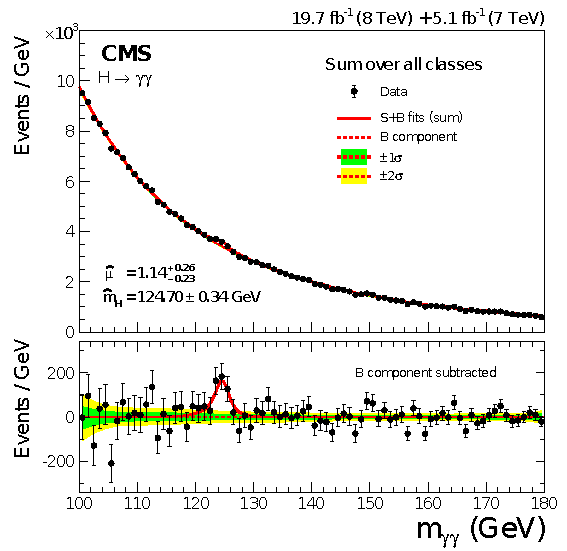
\includegraphics{results.pdf}
    \end{center}
    \caption{The sum of 25 signal plus background fits showing an excess at $m_{\gamma\gamma} = 125.7$ GeV. The lower portion shows the residual after subtracting the background portion of the fit}
    \label{fig:results}
\end{figure}

The diphoton mass spectrum shows an excess with a best fit mass of $124.70\pm 0.34$ GeV.
The largest uncertainties come from possible differences between \hgg and $Z\rightarrow e^+e^-$ which is used to determine the efficiencies  of the photon trigger, reconstruction, and identification as wells as energy scales and corrections.
Differences in the electron and photon response of the detector, non-linearity in the energy scale going form $Z$ bosons to the Higgs Boson, and energy scale calibration and resolution.
The analysis was also able to put an upper bound on the Higgs with of 2.4 GeV as well as excluding a secondary SM-like Higgs bosons at 95\% confidence level.
All results found are compatible with the SM Higgs theory. 
The Standard Model Higgs boson is compatible with each of the results obtained by this analysis.
%A clear signal is observed in the diphoton channel at a mass of 124.7 GeV with a local significance of 5.7 s, where a significance of 5.2 s is expected for the standard model Higgs boson.  The mass is measured to be 124.70  0.34 GeV = 124.70  0.31 (stat)  0.15 (syst) GeV, and the best-fit signal strength relative to the standard model prediction is 1.14+0.26 ??0.23 = 1.14  0.21 (stat)+0.09 ??0.05 (syst)+0.13 ??0.09 (theo). The best-fit values for the signal strength modifiers associated with the ggH and ttH production mechanisms, and with the VBF and VH mechanisms are found to be �mggH,ttH = 1.13+0.37 ??0.31 and �mVBF, VH = 1.16+0.63 ??0.58.  A direct upper limit on the natural width of the state is set at 2.4 GeV (3.1 GeV expected) at a 95% confidence level, and additional SM-like Higgs bosons are excluded at a 95% confidence level in a large fraction of the mass range between 110 and 150 GeV. The SM spin-0 hypothesis for the observed state is compared to a graviton-like spin-2 hypothesis with minimal couplings.  The hypothesis of the signal being 2+ m is disfavoured. When produced entirely by gluon fusion, it is disfavoured with a 1 ?? CLs value of 94% (92% expected).  All the results are compatible with the expectations from a standard

\section{Endcap Upgrade}

\subsection{High Luminosity LHC}

Around 2023, the LHC will be upgrading to a higher luminosity, dubbed the High Luminosity LHC (HL-LHC).
The peak luminosity will reach $\mathcal{L} = 5\cdot 10^{34} \unit{cm}^{-2}\unit{s}^{-1}$, five times greater than in 2012, with a center of mass energy $\sqrt{s} = $ 14 TeV.
This increased luminosity and energy comes with many complications.
Pileup comes from soft $pp$ collisions that add extra energy to the event.
The HL-LHC will average 140 pileup meaning for each hard interaction there will be around 140 soft interactions that put extra particles into the detector that have to be corrected for.
The current endcap scintillators are becoming opaque from the excessive radiation damage. 
With the upgrade to HL-LHC, the radiation levels will be much higher in this region requiring an upgrade to include radiation hard materials.

\subsection{HGCal}
One proposal for an upgrade to the endcap calorimeter, the High Granularity Calorimeter, is a highly segmented silicon pixel calorimeter.
It has three sections, first an EM silicon section (HGCEE), a front hadronic silicon section (HGCHE), and a back hadronic scintillator section (HGC-S) to catch the tails of the showers.
HGCEE(HGCHE) contains 420(241)$\unit{m}^2$ of 300 $\mu$m thick silicon wafers, 6.0M(2.7M) channels and 30(12) layers.
The layers of silicon are separated by tungsten and copper absorber in HGCEE and brass absorber in HGCHE.
Electromagnetic showers in HGCal has a Moli\`{e}re radius containing 90\% of energy of 28 mm and a resolution of about $20\%/\sqrt{E(\textrm{GeV})}$. 
Compared to other upgrade options, the resolution is much worse, but the segmentation allows from corrections never before done in CMS. 
The granularity and low Moli\`{e}re radius make the detector better at handling pileup and provides a good measurement of the position and angle of the particle. 

Using Monte Carlo generated with a model of the new detector, we can predict the mass resolution of the Higgs boson using photons reconstructed in the upgraded endcap.
For this test, 1000 Higgs diphoton decays were simulated at 140 pileup. 
Around 30\% of events include one photon in the barrel and one in the endcap. 


\begin{figure}[h]
    \begin{center}
        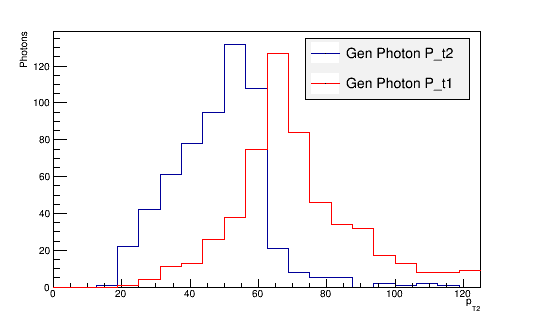
\includegraphics[width=\textwidth]{gen_pt.png}
    \end{center}
    \caption{Photon $p_T$ in HGCal for \hgg, highest $p_T$ in red and secondary in blue.}
    \label{fig:kin}
\end{figure}

The truth particles are matched to reconstructed photons in the barrel and to energy clusters in HGCal. 
The clusters are collections of energy deposits in HGCal optimized to match tracks of charged particles and to group energy deposits that come from the same incident particle.
Energy deposits are calibrated to sum to the total energy of a particle shower.
The calibration for electromagnetic showers in HGCal is performed using single particle gun Monte Carlo.

A muon gun sample is used to determine a scale factor for the different types of active material in the detector.
A Landau function is fit to the energy deposits per cell to give the most probable value of energy a minimum ionizing particle (MIP) leaves in the cell.
This allows us to compare the simulated energy deposited in different thicknesses of silicon wafers and to the energy in the plastic scintillator. 
For a photon gun event, the energy is first scaled by the MIP value and then by the amount of absorber in front of the particular layer $w_i$ to account for the energy that is deposited in the absorber.  
The calibration constant $C$ is determined by a linear fit of the total weighted MIPs by the generated energy. Equation \ref{eq:cal} summarizes the calculation of the reconstructed energy $E_{rec}$. 

\begin{equation}
    E_{rec} =  C \sum_i \frac{E_i w_i }{\textrm{MIP}_i}
    \label{eq:cal}
\end{equation}

For $pp$ events with pileup, there will be much more than one particle at a time in the detector.
This is where the granularity of HGCal can be used to improve the association of hits in the detector with particles from the event. 
A clustering algorithm is used to group hits in the detector that originated from the same source.
Previous algorithms used only the spatial distribution of hits to determine which should be associated, but the higher granularity resulted in more clusters per than particles.
A new algorithm was implemented that takes into account the expected shape of an electromagnetic shower. 
These showers have a high energy peak that falls off exponentially around the center.
After a seed cell is found, hits are added to the cluster as long as the energy is decreasing or the shower width is 1.5 times the Moli\`{e}re radius. 

\begin{figure}[h]
    \begin{center}
        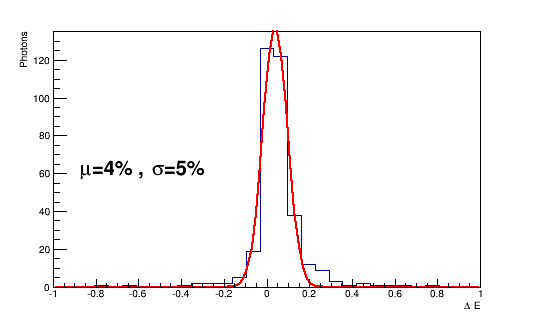
\includegraphics[width=\textwidth]{en_diff.png}
    \end{center}
    \caption{Percent error of reconstructed energy of photons in and HGCal}
    \label{fig:res}
\end{figure}

Photons that have converted to a $e^+ e^-$ pair will show up in HGCal as multiple clusters matched to electron tracks or clusters with a large spread in energy, however, for simplicity, converted photons are removed from this analysis by requiring the cluster seed energy to be greater 95\% of the cluster energy.
Also, we require that the transverse momentum of the photons be greater than 20 GeV.
Figure \ref{fig:res} shows the percent difference of the reconstructed and generated energy for photons in the endcap.
On average the reconstructed energy is 4\% lower than the generated energy with a standard deviation of 5\%. 

The diphoton invariant mass for events with one barrel photon and one endcap photon shown in Figure \ref{fig:mass_spec} has a width of 4.3 GeV.
For comparison, \ref{fig:mass_spec_bb} shows the invariant mass for two photons in the barrel with a width of 4.0 GeV.
It is important to note that these resolutions are a baseline that can be improved upon using many known techniques, such as pileup subtraction for reducing the impact of pileup on the measured energies.
Also, the photons that are reconstructed in the barrel have not been optimized for the high pileup scenario. 

\begin{figure}[h]
    \begin{center}
            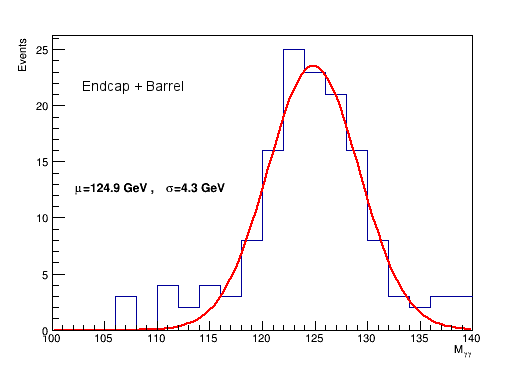
\includegraphics[width=\textwidth]{higgs_mass.png}
    \end{center}
    \caption{$M_{\gamma\gamma}$ spectrum from Higgs decay for one endcap and one barrel photon}
    \label{fig:mass_spec_bb}
\end{figure}
\begin{figure}[h]
    \begin{center}
        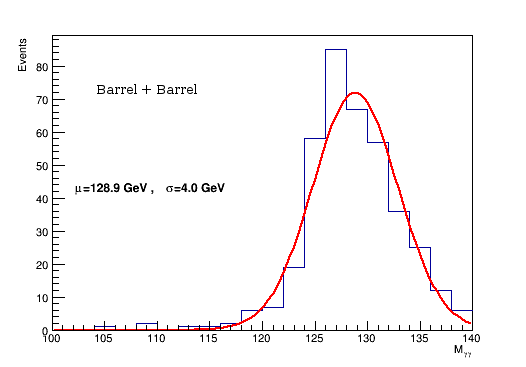
\includegraphics[width=\textwidth]{higgs_massB+B.png}
    \end{center}
    \caption{$M_{\gamma\gamma}$ spectrum from Higgs decay for two barrel photons}
    \label{fig:mass_spec}
\end{figure}

\section{Conclusion}

The Higgs mechanism is a foundational part the Standard Model which has been solidified by the observation of the Higgs decay to photons by the CMS.
As the LHC upgrades to higher luminosities necessary to further search for particles beyond the standard model, the CMS must upgrade to survive the higher radiation and pileup.
Through this simple analysis of simulated events, HGCal is shown to be able to measure the energy of photons to provide a reasonable Higgs mass resolution of 4.3 GeV which could improve with better treatment of pileup. 

My further work on HGCal will be working with a team testing and developing methods for measuring hadronic showers, continuing to deal with the high pileup scenario of the HL-LHC.


\bibliography{checking}{}
\bibliographystyle{plain}
\end{fmffile}
\end{document}
